%
% File naaclhlt2016.tex
%

\documentclass[11pt,letterpaper]{article}
\usepackage{naaclhlt2016}
\usepackage{times}
\usepackage{latexsym}
\usepackage{url}
\usepackage{latexsym}
\usepackage{float}
\usepackage{graphicx} 
\usepackage{subfigure}

\naaclfinalcopy % Uncomment this line for the final submission
\def\naaclpaperid{***} %  Enter the naacl Paper ID here

\newcommand\BibTeX{B{\sc ib}\TeX}

\title{Human Gender and Facial Expression Classification}

\author{Jifu Zhao (jzhao59)\\
	    Depart of Nuclear, Plasma, and Radiological Engineering\\
	    104 South Wright Street\\
	    Urbana, IL 61801, USA\\
	    {\tt jzhao59@illinois.edu}}

\date{}

\begin{document}

\maketitle

\begin{abstract}
Human gender and facial expressions is an important way for humans to commutate with others. In this paper, based on the collected human face pictures, we apply a series of machine learning algorithms to solve this multi-classification problem.
\end{abstract}

\section{Introduction}

Pictures is an important way for humans to communicate with the world. Especially now, with the development of modern social media, such as Facebook, Instagram and so on, people tend to express their emotions through social media. With so many information online, it is needed to make the machines to learn how to classify the pictures based on gender, facial expressions and so on.\\

Normally, there are only males and females. But people can have multiple facial expressions, such as smile, non-smile, angry, sad, scared and so on. So, the final goal is to teach the machines to learn how to accurately classify these expressions. However, the available dataset is limited. So, in this paper, we address one simple situation: classify pictures into four categories according to gender and smile or non-smile facial expressions.\\

This paper will apply different learning algorithms towards the same data. And compare the learning algorithms in original feature space as well as in reduced dimensionality feature space. The result will be shown through some statistical validation.\\

More precisely, this paper can be divided into the following sections. Section 2 describes the dataset and problem to be solved. Section 3 will talk about the methods that will be used in this paper to reduce the dimensionality. Section 4 will talk about the algorithms that will be used to solve this multi-classification problem. Section 5 will show the result. And Finally, section 6 will summarize the whole paper.\\

\section{Dataset and Problem Description}

To successfully address this multi-classification problem, the appropriate dataset is crucial. After some study on available image dataset, we finally decided to use the FEI Face Database (Thomaz and Giraldi, 2010). The FEI face database (\url{http://fei.edu.br/~cet/facedatabase.html}) is a Brazilian face database that contains a set of face images for 200 individuals, including 100 males and 100 females. These pictures is divided into different types based on their information, such as in color scale or in gray scale, only frontal face part or with background information. In this project, we use three subsets of the original images.\\

The first one is the smallest images: only the frontal face images, as shown in figure 1, which is called {\bf cropped-faces}. The second one is also the gray scale images, but this time there will be more information, such as hair and so on. The sample pictures are shown in figure 2, which is called {\bf gray-faces}. And the third subset, which contains the images in RGB format, contains all the information. This subset is called {\bf color-faces}, as shown in figure 3.\\

\begin{figure}[H]
\centering
\subfigure[Non-smile]{
\label{Fig.sub.1}
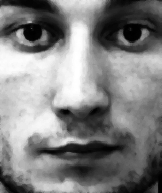
\includegraphics[width=0.2\textwidth]{2alittle.jpg}}
\subfigure[Smile]{
\label{Fig.sub.2}
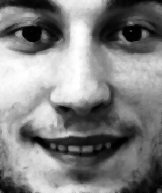
\includegraphics[width=0.2\textwidth]{2blittle.jpg}}
\caption{Cropped faces}
\label{Fig.lable}
\end{figure}

\begin{figure}[H]
\centering
\subfigure[Non-smile]{
\label{Fig.sub.1}
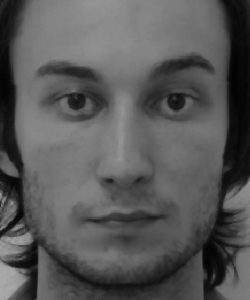
\includegraphics[width=0.2\textwidth]{2afront.jpg}}
\subfigure[Smile]{
\label{Fig.sub.2}
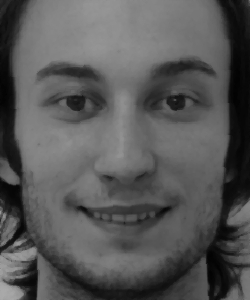
\includegraphics[width=0.2\textwidth]{2bfront.jpg}}
\caption{Gray faces}
\label{Fig.lable}
\end{figure}

\begin{figure}[H]
\centering
\subfigure[Non-smile]{
\label{Fig.sub.1}
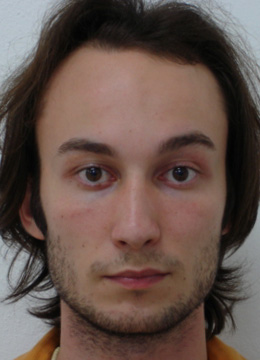
\includegraphics[width=0.2\textwidth]{2a.jpg}}
\subfigure[Smile]{
\label{Fig.sub.2}
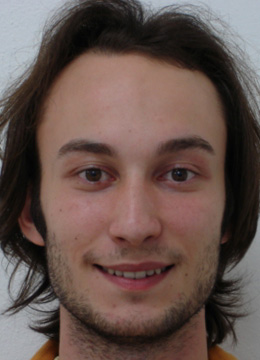
\includegraphics[width=0.2\textwidth]{2b.jpg}}
\caption{Color faces}
\label{Fig.lable}
\end{figure}

There will be 400 images in each subset, and 200 individuals with smile expressions and the other 200 individuals with non-smile expressions. So, for each subset, there will be 100 men with smile expressions, 100 men with non-smile expressions, 100 women with smile expressions, and 100 women with non-smile expressions. Using these 400 images, we can finish this multi-classification problem.\\

Given these pictures, we want to answer the following questions:

\begin{enumerate}
\item[1, ] Which algorithm is best for this problem?
\item[2, ] What's the influence of different kinds of pictures?
\item[3, ] what's the difference between original feature space and reduced dimensionality feature space?
\end{enumerate}

For problem 1, we will compare 4 different algorithms: Linear Discriminant Analysis (LDA), K-nearest Neighboors, Support Vector Machines (SVM) with rbf kernel and linear kernel. For problem 2, we will compare the results on these three subsets. For problem 3, we will use Principal Component Analysis (PCA) to reduced the dimensionality and compare the results in PCA space and original space.\\

\section{Dimensionality Reduction}

The pictures have been manually labelled into 4 classes: man smile, man non-smile, woman smile, and woman non-smile. In order to apply machine learning method, we need to have training set and test set. So, the original data set is randomly shuffled. Then, $75\%$ ($300$ faces) are randomly selected as the training set, and the rest $25\%$ ($100$ faces) are chosen as the test set. This process is repeated three times for all three subsets. In order to compare the influence of the information contained in pictures, we select the same pictures as training set for all three subsets.\\

All pictures will be vectorized in to column vectors to form a matrix. So, for this matrix, every column is one picture, and each row is one feature. In this question, the features for three different pictures (cropped-faces, gray-faces, and color-faces) are as follows:\\
\begin{center}
$193 \times 162 = 31266$\\
$300 \times 250 = 75000$\\
$360 \times 260 \times 3 = 280800$\\
\end{center}

As mentioned above, we will use PCA method to reduce the dimensionality. In PCA method, the first step is to center the data, this process can be done by easily subtracting the mean faces. After center the data, the mean faces are shown in Figure 4. Since we choose the same pictures as the training set, all three mean faces look similar.\\

\begin{figure}[H]
\centering
\subfigure[frontal face]{
\label{Fig.sub.1}
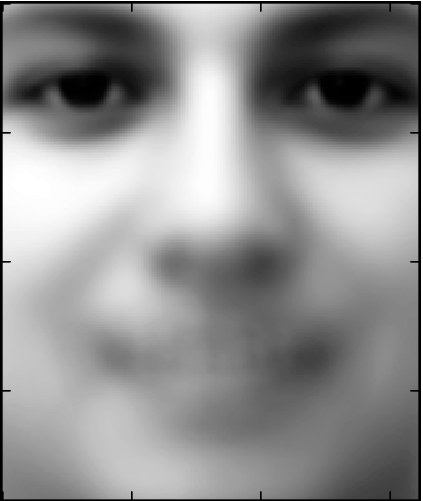
\includegraphics[width=25mm, height=30mm]{meanFace.png}}
\subfigure[full face]{
\label{Fig.sub.1}
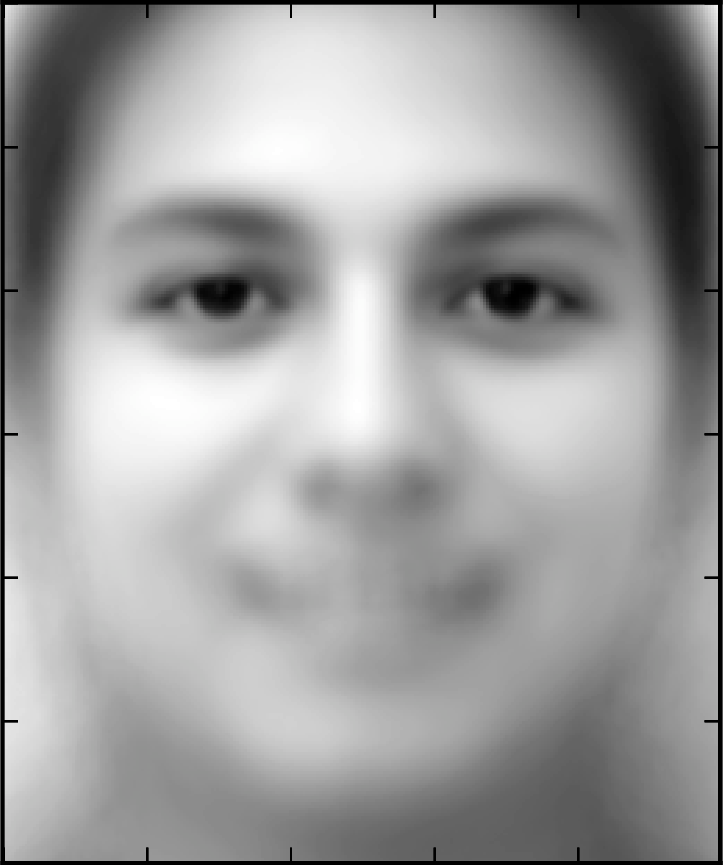
\includegraphics[width=25mm, height=30mm]{meanFace2.png}}
\subfigure[colored face]{
\label{Fig.sub.2}
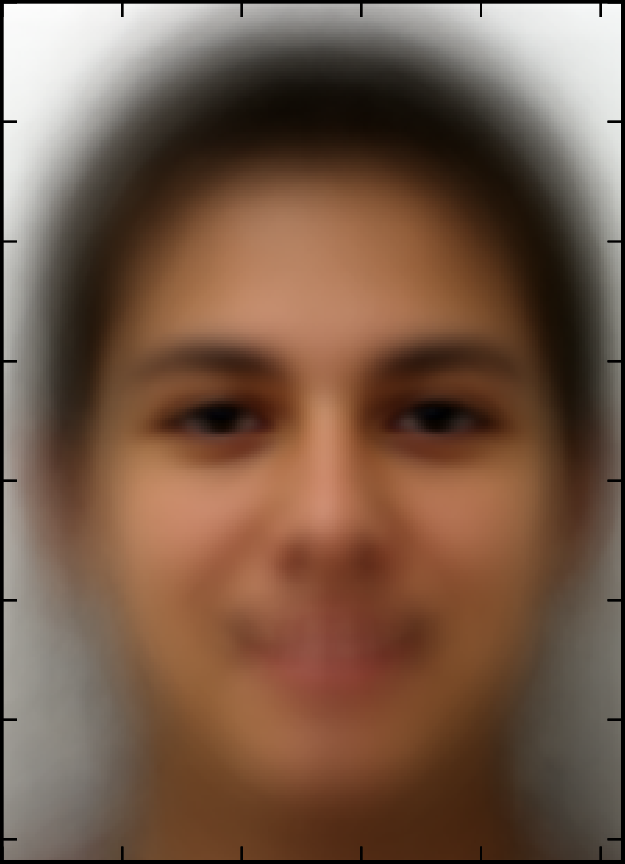
\includegraphics[width=23mm, height=30mm]{meanFace3.png}}
\caption{Mean faces}
\label{Fig1.lable}
\end{figure}

Having centered the data, next we can perform the PCA through Singular value decomposition (SVD) over the covariance matrix. Since this process is the same for three subsets, we will only show the results of the cropped-faces. \\

Through PCA, we can get a series of eigenvectors. These eigenvectors can be seen as the eigen-faces, which can be used to reproduce the original faces. A sample of first 16 eigen-faces are shown in Figure 5.\\

\begin{figure}[H]
\centering
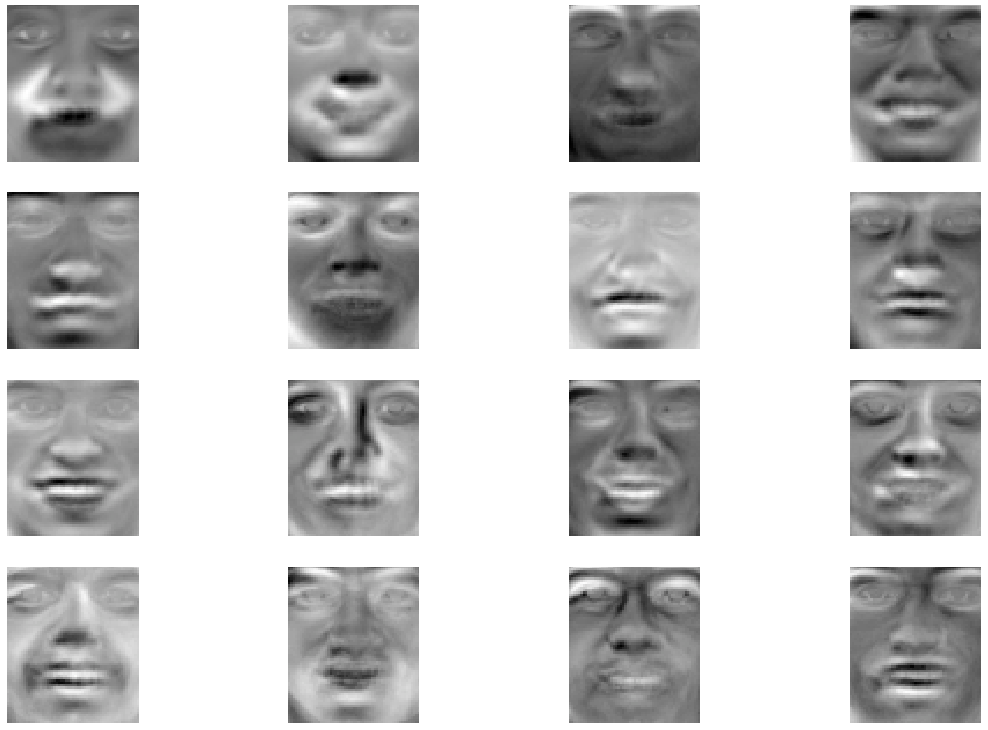
\includegraphics[width=80mm]{eigenFace.png}
\caption{Eigen-faces}
\label{Fig2.lable}
\end{figure}

The corresponding explained variance ratio, which measures the relative significance of the eigen-faces, is shown in Figure 6.\\

\begin{figure}[H]
\centering
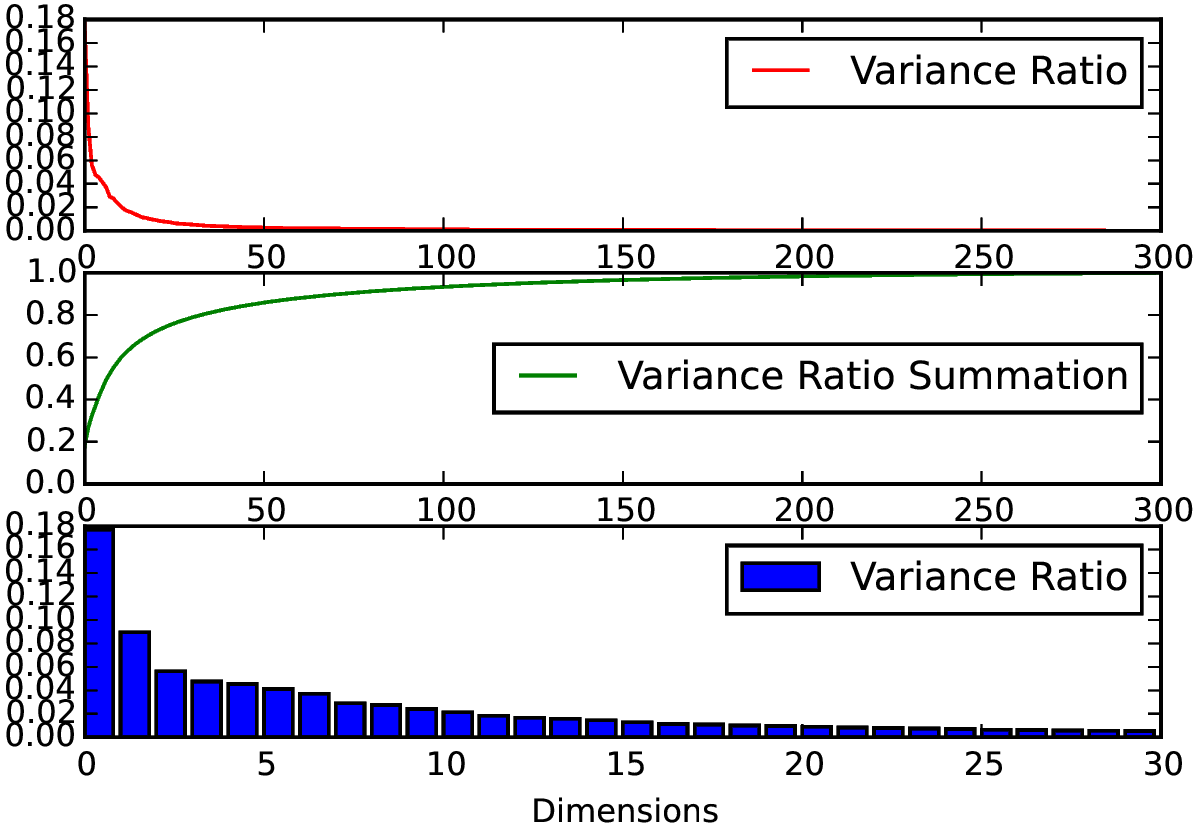
\includegraphics[width=85mm]{ratioChange.png}
\caption{Explained variance ratio}
\label{Fig2.lable}
\end{figure}

As shown in figure 6, after performing PCA, the original feature space, which contains $31266$ features, can be reduced to the PCA space with less features. For example, we can use $80\%$, $90\%$ or $95\%$ of the total information to represent the original pictures. Although we will lose some information, our feature space can be dramatically reduced, which will help to save the computation time.\\

After PCA, we got a series of eigen-faces. These eigen-faces can be used to reconstruct the original faces. If we project the original pictures on the eigen-faces, we can see some boundary information. To show this clearly, we use the first two eigen-faces, and project the cropped-faces, gray-faces and color-faces on the corresponding first two eigen-faces. The results are shown in figure 7, 8, 9.\\

Comparing figure 7, 8 and 9, we can see some difference. In figure 7, the boundary between smile and non-smile (including woman and man) is relatively clear, but the boundary between man and women is not clear at all. But in figure 8 and 9, the boundary between man and woman is much more clear than the boundary between smile and non-smile, which is totally different from figure 7.

\begin{figure}[H]
\centering
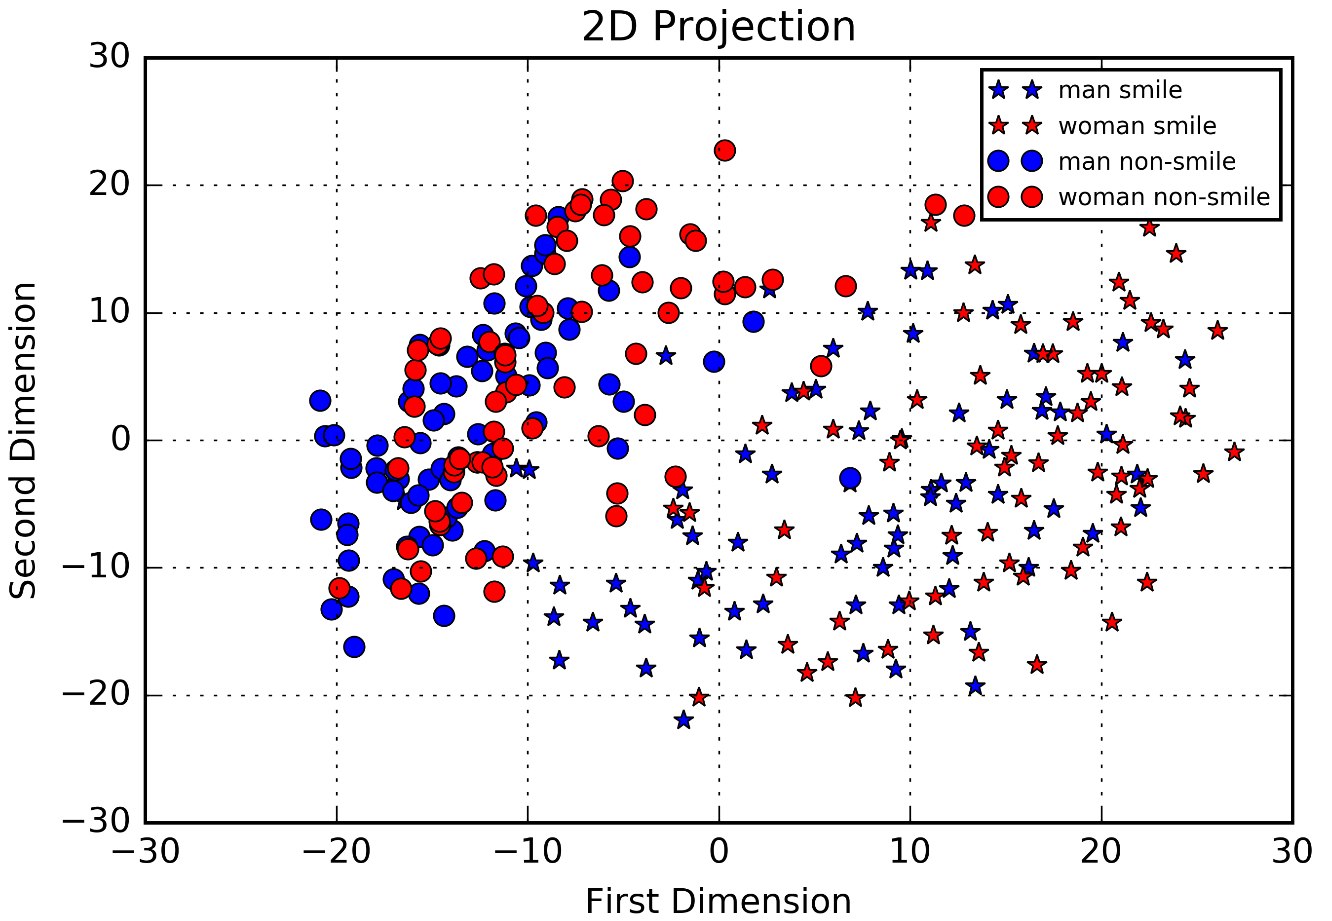
\includegraphics[width=81mm]{little_2dProjection.png}
\caption{Cropped faces projection}
\label{little.lable}
\end{figure}

\begin{figure}[H]
\centering
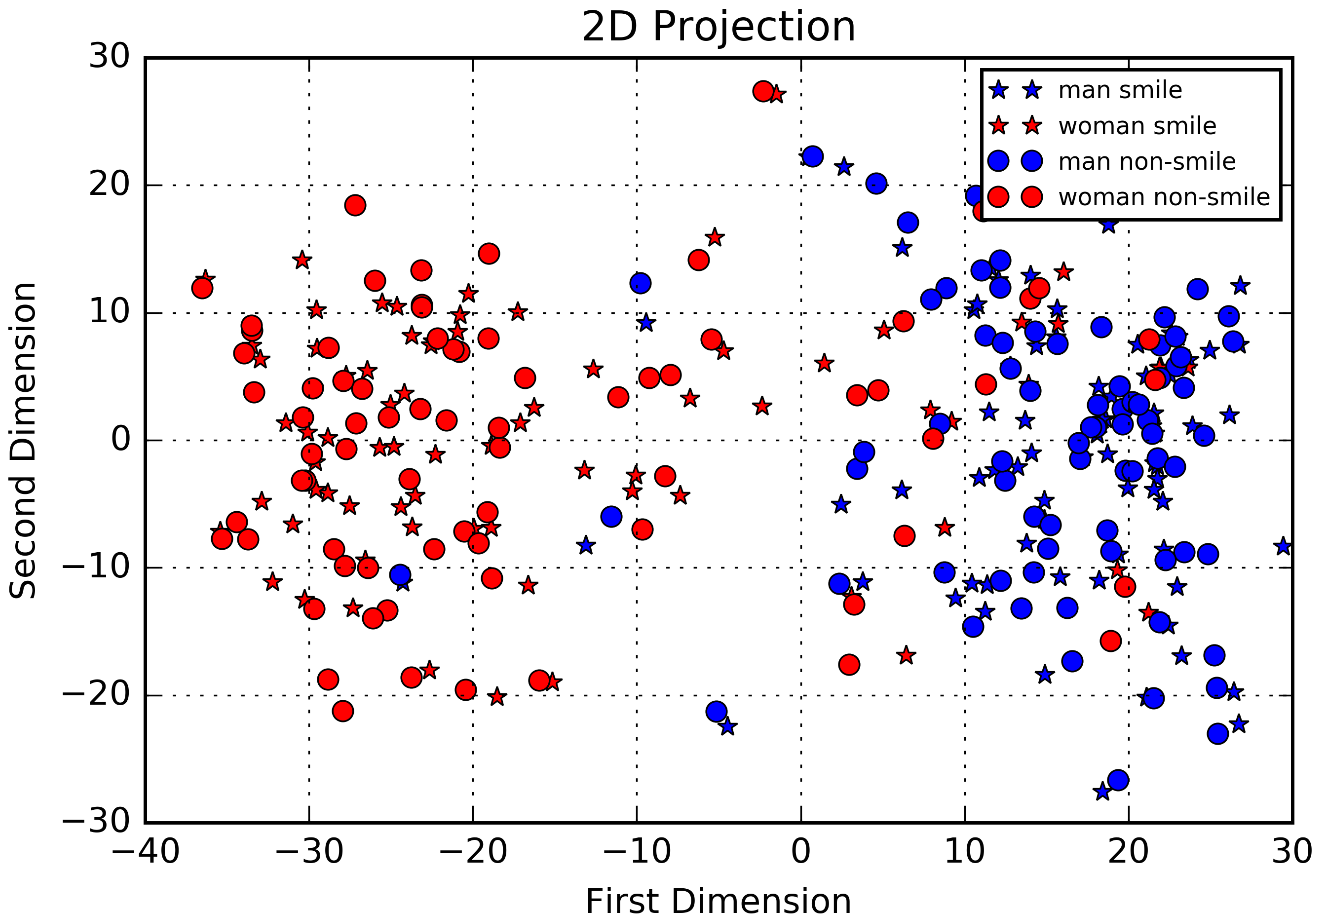
\includegraphics[width=81mm]{front_2dProjection.png}
\caption{Gray faces projection}
\label{front.lable}
\end{figure}

\begin{figure}[H]
\centering
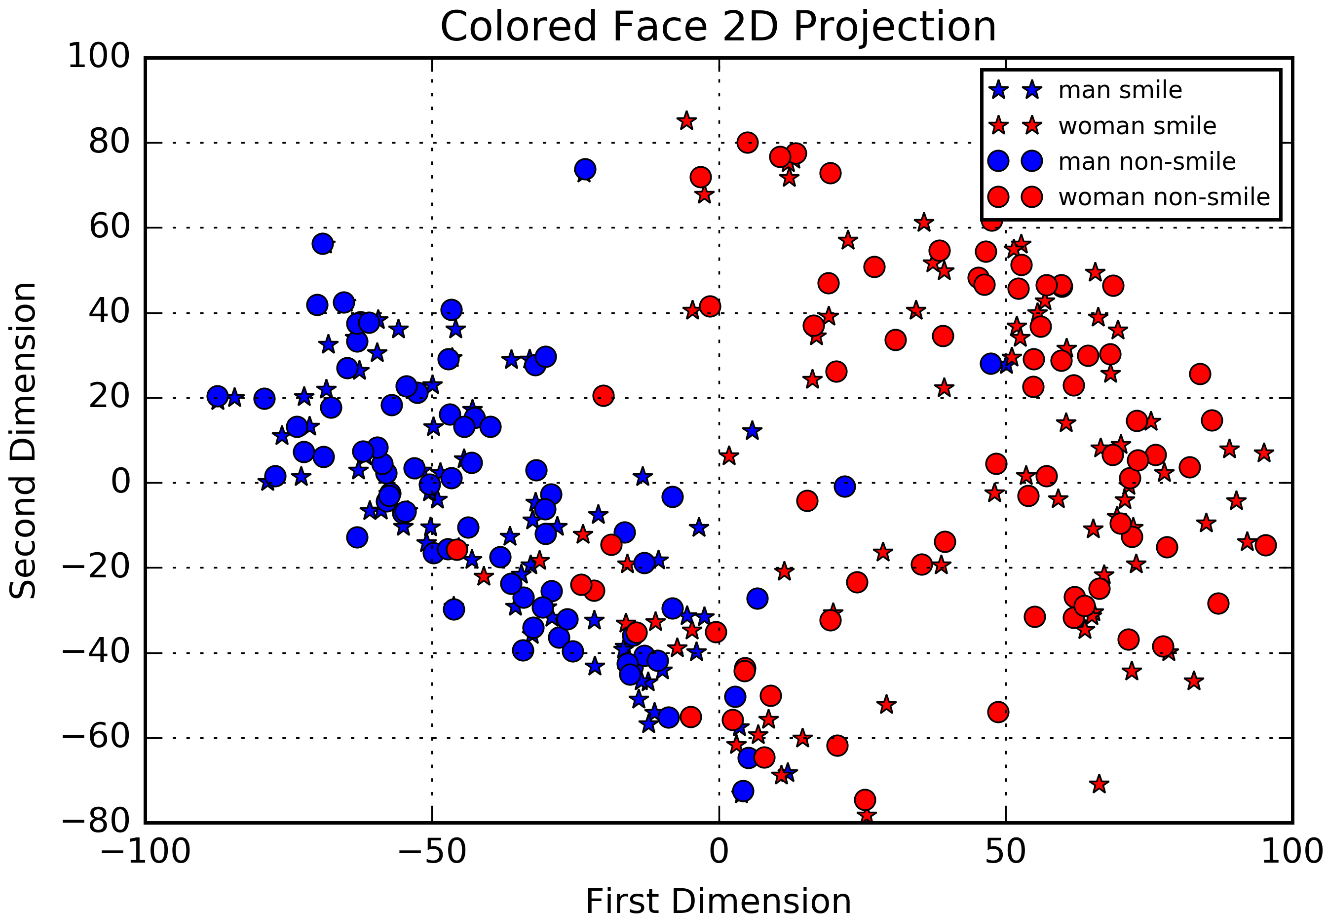
\includegraphics[width=81mm]{color_2dProjection.png}
\caption{Color faces projection}
\label{Fig_color.lable}
\end{figure}

This phenomenon is because that in cropped-faces, we only keep the frontal face information, in which the difference between woman and man is not clear, but the difference between smile and non-smile is not clear. However, in gray-faces and color-faces, we not only have the information about frontal face, but also have information about hair and so on. So, this time, the difference between man and woman is clear, but the difference between smile and non-smile expressions is not clear.\\

Another clear difference is that, as the feature space increases (from figure 7 to figure 9), it will be harder and harder to find the clear boundaries for these 4 categories. This is because that as feature numbers increase, there will be more and more useless information, which can be seen as the noise. These useless information will reduce the classification accuracy. \\

\section{Learning Algorithms}
For multi-classification problems, we can use One-vs-All or All-vs-All principals. We tried a series of learning algorithms, from the Linear Discriminant Analysis (LDA), Quadratic Discriminant Analysis (QDA), to Decision Trees, K-nearest Neighboors(KNN), Support Vector Machines (SVM) with rbf kernel, linear kernel and polynomial kernel. Having Observed their accuracy on the training set and test set, we finally decided to choose LDA, KNN (k=5 in this paper), SVM with rbf kernel and SVM with linear kernel learning algorithms.\\

In addition, since we only have 400 pictures for each subset, to make our result to be more persuasive, we choose 5 folder cross validation. So, every result is the average value of the 5 different accuracies.\\

\section{Results and Discussion}

Having successfully prepared the data and decided the learning algorithms, we can perform the classification now. \\

Firstly, we want to study the effect of different number of PCA features. We change the ratio of the information we want to keep from $10\%$ to $95\%$, train different classifiers and apply them on the training set and test set. The results are shown in figure 10 and 11.\\

\begin{figure}[H]
\centering
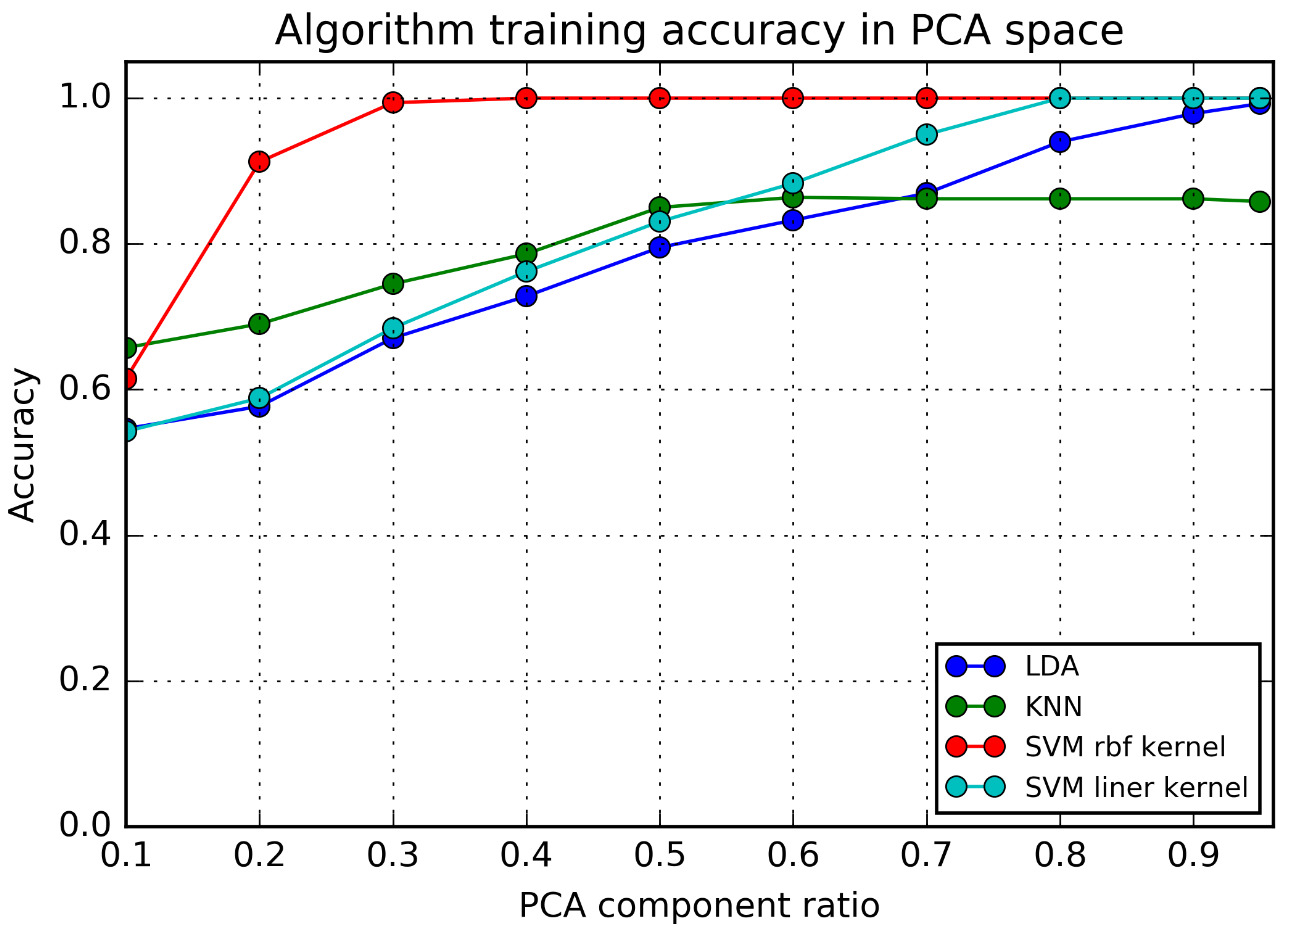
\includegraphics[width=79mm]{little_total_train.png}
\caption{Algorithm training accuracy in PCA space}
\label{train.lable}
\end{figure}

\begin{figure}[H]
\centering
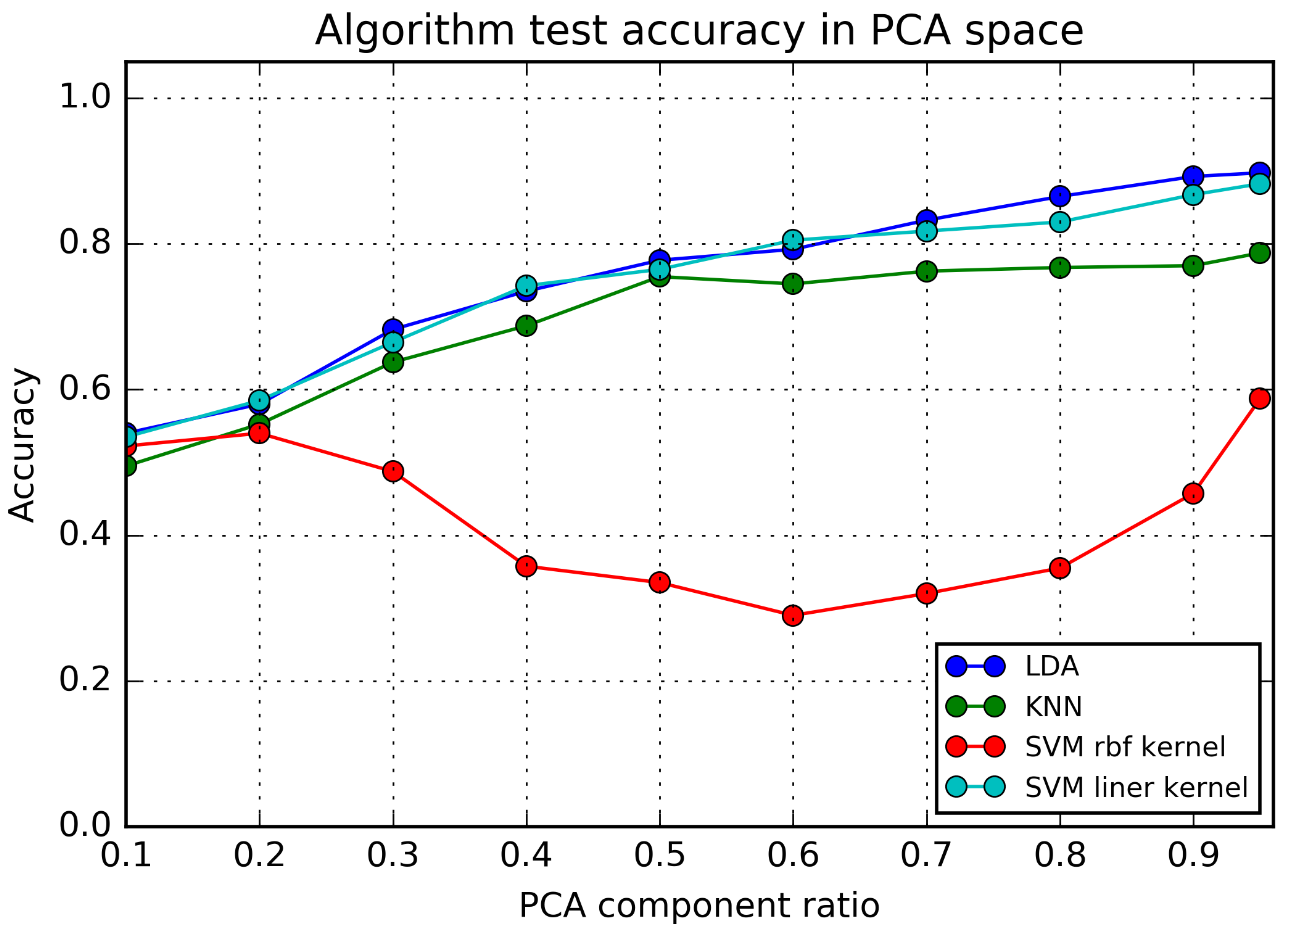
\includegraphics[width=79mm]{little_total_test.png}
\caption{Algorithm test accuracy in PCA space}
\label{test.lable}
\end{figure}

As shown in figure 10, after keeping more than $80\%$ of the total information in PCA space, the SVM with rbf kernel and SVM with linear kernel algorithms can reach $100\%$ accuracy on the training set. LDA and KNN can also reach their highest accuracy on the training set.\\

However, their performance on the test set is different from the training set. With even $95\%$ of the total information, LDA and SVM with linear kernel can reach only $85\%$ accuracy at most. KNN can reach $80\%$ accuracy at most. And SVM with rbf kernel even has a very strange accuracy curve on the test set, about which we haven't found a good explanation.\\

Having found the influence of keeping different ratio of information in PCA space, we can compare the performance of our algorithms on PCA space and original space. Here, we keep $95\%$ of the total information in PCA space. The accuracy on training set and test set is shown in table 1.

%\begin{table}[H]
%  {\centering
%    \begin{tabular}{|c|c||c|c||c|c|}
%      \hline
%& & \multicolumn{2}{c||}{Original space} & \multicolumn{2}{c|}{PCA 95\% space} \\
%\cline{3-6}
%& & training &
% test & training & test \\
%\hline \hline
%& LDA & 0.9794 & 0.9300 & 0.9938 & 0.8750 \\
%\cline{2-6}
%Crop- & KNN & 0.8594 & 0.7825 & 0.8500 & 0.8125 \\
%\cline{2-6}
%ped & SVM rbf & 0.7500 & 0.7275 & 1.0000 & 0.4500 \\
%\cline{2-6}
%faces & SVM linear & 1.0000 & 0.8875 & 1.0000 & 0.8500 \\
%\hline \hline
%
%& LDA & 0.9713 & 0.9050 & 0.9969 & 0.8875 \\
%\cline{2-6}
%Gray & KNN & 0.7188 & 0.7150 & 0.7469 & 0.6250 \\
%\cline{2-6}
%faces & SVM rbf & 0.7588 & 0.7525 & 1.0000 & 0.4250 \\
%\cline{2-6}
%& SVM linear & 1.0000 & 0.8825 & 1.0000 & 0.7875 \\
%\hline \hline
%
%& LDA & 0.9688 & 0.8875 & 0.9875 & 0.8250 \\
%\cline{2-6}
%Color & KNN & 0.6119 & 0.5875 & 0.6063 & 0.5375 \\
%\cline{2-6}
%faces & SVM rbf & 0.6475 & 0.6425 & 1.0000 & 0.2125 \\
%\cline{2-6}
%& SVM linear & 1.0000 & 0.8575 & 1.0000 & 0.7375 \\
%\hline \hline
%
%\end{tabular}
%\caption{Table for Classification results} \label{table:ltu}}
%\end{table}

\begin{table}[H]
  {\centering
    \begin{tabular}{|c|c||c|c||c|c|}
      \hline 
& & \multicolumn{2}{c||}{Original space} & \multicolumn{2}{c|}{PCA 95\% space} \\
\cline{3-6}
& & training &
 test & training & test \\
\hline \hline
& LDA & 0.979 & 0.930 & 0.994 & 0.875 \\
\cline{2-6}
Cro- & KNN & 0.859 & 0.783 & 0.850 & 0.813 \\
\cline{2-6}
pped & SVM rbf & 0.750 & 0.728 & 1.000 & 0.450 \\
\cline{2-6}
faces & SVM linear & 1.000 & 0.888 & 1.000 & 0.850 \\
\hline \hline

& LDA & 0.971 & 0.905 & 0.997 & 0.888 \\
\cline{2-6}
Gray & KNN & 0.719 & 0.715 & 0.747 & 0.625 \\
\cline{2-6}
faces & SVM rbf & 0.759 & 0.753 & 1.000 & 0.425 \\
\cline{2-6}
& SVM linear & 1.000 & 0.883 & 1.000 & 0.788 \\
\hline \hline

& LDA & 0.969 & 0.888 & 0.988 & 0.825 \\
\cline{2-6}
Color & KNN & 0.612 & 0.588 & 0.606 & 0.538 \\
\cline{2-6}
faces & SVM rbf & 0.648 & 0.643 & 1.000 & 0.213 \\
\cline{2-6}
& SVM linear & 1.000 & 0.858 & 1.000 & 0.738 \\
\hline \hline

\end{tabular}
\caption{Table for Classification results} \label{table:ltu}}
\end{table}

As shown in table 1, generally, all these algorithms have better performance in the original space than the PCA space, especially when the feature space is enlarged. When the feature space is increased, the accuracy of 4 algorithms will decrease in both original space and PCA space. \\

More specifically, although SVM with linear kernel algorithm has very good performance on training set in original space and PCA space, LDA has higher accuracy on test set than SVM with linear kernel.\\

\section{Conclusions}

Through the above analysis, it is easy to answer the questions put forward at the beginning:
\begin{enumerate}
\item[1, ] LDA algorithm has better overall performance than other algorithms for this question.
\item[2, ] As there are more and more information, the accuracy of all 4 algorithms will decrease. 
\item[3, ] All 4 algorithms have higher accuracies in the original space than PCA space.
\end{enumerate}

As shown above, PCA method can reduce the feature space and help to save the computation time, but it will also decrease the accuracy of different algorithms than in original feature space.\\

Comparing the results on three subsets, it is always desirable to have the cropped images. This subset has not only higher accuracy, but also less computation time. But in order to get the cropped images, we need some other techniques to process the images before the classification.\\

This paper is based on the sample of 400 pictures. This makes it hard to fully reflect the real world images. There are still a lot of related works to be done.\\

%\bibliography{naaclhlt2016}
%\bibliographystyle{naaclhlt2016}
\begin{thebibliography}{}

\bibitem[\protect\citename{Thomaz and Giraldi}2010]{Aho:72}
C. E. Thomaz and G. A. Giraldi.
\newblock 2010.
\newblock {\em A new ranking method for Principal Components Analysis and its application to face image analysis}, volume~28.
\newblock Image and Vision Computing.

\bibitem[\protect\citename{Theodoridis and Koutroumbas}2009]{Aho:72}
S. Theodoridis and K. Koutroumbas
\newblock 2009.
\newblock {\em Pattern Recognition (Fourth Edition)}, 
\newblock Elsevier Inc.

\bibitem[\protect\citename{Theodoridis and Koutroumbas}2009]{Aho:72}
M. A. Turk and A. P. Pentland
\newblock 1991.
\newblock {\em Face Recognition Using Eigenfaces}, 
\newblock Computer Vision and Pattern Recognition.

\bibitem[\protect\citename{Delac, Grgic and Grgic}2006]{Aho:72}
K. Delac, M. Grgic and S. Grgic
\newblock 2006.
\newblock {\em Independent Comparative Study of PCA, ICA, and LDA on the FERET Data Set}, 
\newblock International Journal of Imaging Systems and Technology.

\end{thebibliography}

\end{document}
